\documentclass{standalone}
\usepackage{ebgaramond-maths}
\usepackage{tikz}
\definecolor{V}{RGB}{148,0,0}
\def\Xscale{16}
\def\Yscale{9}
\def\Xfactor{0.9}
\def\Yfactor{0.9}
\def\Xshift{1.3}
\def\Yshift{0.4}
\def\TotalP{20}
\begin{document}
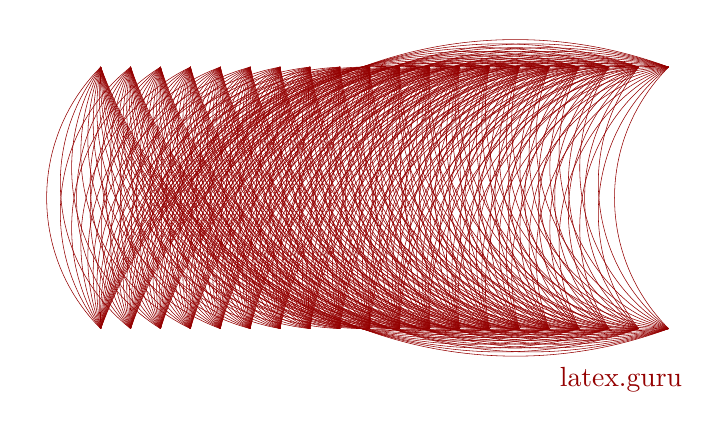
\begin{tikzpicture}[x=15pt,y=15pt]
    \path[use as bounding box] (0,0) rectangle (\Xscale,\Yscale);
    \foreach \P in {1,...,\TotalP} {
        \coordinate (B\P) at ({\Xfactor*\P*\Xscale/\TotalP+\Xshift*\Xscale/\TotalP},{\Yfactor*1.5+\Yshift});
        \coordinate (T\P) at ({\Xfactor*\P*\Xscale/\TotalP+\Xshift*\Xscale/\TotalP},{\Yfactor*8.5+\Yshift});
    }
    \foreach \B in {1,...,\TotalP} {\foreach \T in {1,...,\TotalP} {\draw[V,line cap=round,line width=0.2pt] (B\B)to[bend left=45](T\T);}}
    \node[V,anchor=south east] at (current bounding box.south east) {latex.guru};
\end{tikzpicture}
\end{document}